\documentclass{article}
\usepackage[utf8]{inputenc} %кодировка
\usepackage[T2A]{fontenc}
\usepackage[english,russian]{babel} %русификатор 
\usepackage{mathtools} %библиотека матеши
\usepackage[left=1cm,right=1cm,top=2cm,bottom=2cm,bindingoffset=0cm]{geometry} %изменение отступов на листе
\usepackage{amsmath}
\usepackage{graphicx} %библиотека для графики и картинок
\graphicspath{}
\DeclareGraphicsExtensions{.pdf,.png,.jpg}
\usepackage{subcaption}
\usepackage{pgfplots}
\usepackage{float}
\usepackage{listings}
\usepackage{hyperref}
\usepackage{physics}
\usepackage{xcolor}

\lstset{language=Java,
        basicstyle=\ttfamily,
        keywordstyle=\color{blue}\ttfamily,
        stringstyle=\color{red}\ttfamily,
        commentstyle=\color{green}\ttfamily,
        morecomment=[l][\color{magenta}]{\#},
        captionpos=b,
        frame=single % рамка вокруг кода
}

\begin{document}
% НАЧАЛО ТИТУЛЬНОГО ЛИСТА
\begin{center}
    \Large
    Федеральное государственное автономное \\
    образовательное учреждение высшего образования \\ 
    «Научно-образовательная корпорация ИТМО»\\
    \vspace{0.5cm}
    \large
    Факультет программной инженерии и компьютерной техники \\
    Направление подготовки 09.03.04 Программная инженерия \\
    \vspace{1cm}
    \Large
    \textbf{Отчёт по лабораторной работе №6} \\
    По дисциплине «Вычислительная математика» (4 семестр)\\
    \large
    \vspace{8cm}

    \begin{minipage}{.33\textwidth}
    \end{minipage}
    \hfill
    \begin{minipage}{.4\textwidth}
    
        \textbf{Студент}: \vspace{.1cm} \\
        \ Дениченко Александр P3212\\
        \textbf{Практик}:  \\
        \ Наумова Надежда Александровна
    \end{minipage}
    \vfill
Санкт-Петербург\\ 2024 г.
\end{center}
\pagestyle{empty}
% КОНЕЦ ТИТУЛЬНОГО ЛИСТА 
\newpage
\pagestyle{plain}
\section{Цель работы}
Решить задачу интерполяции, найти значения функции при заданных значениях аргумента, отличных от узловых точек.
\section{Машинная реализация}
\begin{lstlisting}[caption={Реализация метода Адамса.}]
public List<String> solve(DifferentialEquation eq, double x0, double y0, 
double xn, double h, double eps) {
    List<String> points = new ArrayList<>();
    double[] y = new double[ORDER];
    double[] x = new double[ORDER];
    y[0] = y0;
    x[0] = x0;
    points.add("(" + formatScientificNotation(x[0]) + ", " 
    + formatScientificNotation(y[0]) + ")");
    for (int i = 1; i < ORDER; i++) {
        double h1 = h;
        boolean acceptStep = false;
        while (!acceptStep) {
            double k1 = h1 * eq.eval(x[i-1], y[i-1]);
            double k2 = h1 * eq.eval(x[i-1] + h1 / 2, y[i-1] + k1 / 2);
            double k3 = h1 * eq.eval(x[i-1] + h1 / 2, y[i-1] + k2 / 2);
            double k4 = h1 * eq.eval(x[i-1] + h1, y[i-1] + k3);
            double yNext = y[i-1] + (k1 + 2 * k2 + 2 * k3 + k4) / 6;

            double halfStep = h1 / 2;
            double k1_half = halfStep * eq.eval(x[i-1], y[i-1]);
            double k2_half = halfStep * eq.eval(x[i-1] + halfStep / 2, y[i-1] +
            + k1_half / 2);
            double k3_half = halfStep * eq.eval(x[i-1] + halfStep / 2, y[i-1] + 
            +k2_half / 2);
            double k4_half = halfStep * eq.eval(x[i-1] + halfStep, y[i-1] + k3_half);
            double yHalfStep = y[i-1] + (k1_half + 2 * k2_half + 2 * k3_half +
            + k4_half) / 6;

            double R = Math.abs(yNext - yHalfStep) / (Math.pow(2, 4) - 1);

            if (R <= eps) {
                acceptStep = true;
                y[i] = yNext;
                x[i] = x[i-1] + h1;
                points.add("(" + formatScientificNotation(x[i]) + ", " +
                + formatScientificNotation(y[i]) + ")");
            } else {
                h1 *= 0.5;
            }
        }
    }
    double maxError = 0;
    while (x[ORDER - 1] < xn) {
        double fI = eq.eval(x[ORDER - 4], y[ORDER - 4]);
        double fI1 = eq.eval(x[ORDER - 3], y[ORDER - 3]);
        double fI2 = eq.eval(x[ORDER - 2], y[ORDER - 2]);
        double fI3 = eq.eval(x[ORDER - 1], y[ORDER - 1]);
        double deltaFI = fI3 - fI2;
        double delta2FI = fI3 - 2*fI2 + fI1;
        double delta3FI = fI3 - 3*fI2 + 3*fI1 - fI;
        double yNext = y[ORDER - 1] + h*fI3 + Math.pow(h, 2)*0.5*deltaFI +
        + 5/12.f*Math.pow(h, 3)*delta2FI + 3/8.f*Math.pow(h, 4)*delta3FI;
        maxError = Math.max(maxError, Math.abs(eq.getYRight(x0, y0, x[ORDER - 1])-
         - yNext));
        System.arraycopy(x, 1, x, 0, ORDER - 1);
        System.arraycopy(y, 1, y, 0, ORDER - 1);
        x[ORDER - 1] += h;
        y[ORDER - 1] = yNext;
        points.add("(" + formatScientificNotation(x[ORDER - 1]) + ", "+
         + formatScientificNotation(y[ORDER - 1]) + ")");
    }
    if(maxError < eps){
        return points;
    }else return solve(eq,  x0, y0, xn, h*0.5, eps);
}
\end{lstlisting}

\begin{lstlisting}[caption={Реализация метода Рунге-Кутты 2 порядка.}]
public List<String> solve(DifferentialEquation eq, double x0, double y0, 
double xn, double h, double eps) {
    List<String> points = new ArrayList<>();
    double y = y0;
    double x = x0;
    points.add("("+formatScientificNotation(x)+", "+formatScientificNotation(y)+")");

    while (x < xn) {
        if (x + h > xn) h = xn - x;  
        double k1 = h * eq.eval(x, y);
        double k2 = h * eq.eval(x + h / 2, y + k1 / 2);
        double k3 = h * eq.eval(x + h / 2, y + k2 / 2);
        double k4 = h * eq.eval(x + h, y + k3);
        double yNext = y + (k1 + 2 * k2 + 2 * k3 + k4) / 6;

        double k1H = 0.5 * h * eq.eval(x, y);
        double k2H = 0.5 * h * eq.eval(x + h / 4, y + k1 / 2);
        double k3H = 0.5 * h * eq.eval(x + h / 4, y + k2 / 2);
        double k4H = 0.5 * h * eq.eval(x + h / 2, y + k3);
        double yHalfStep = y + (k1H + 2 * k2H + 2 * k3H + k4H) / 6;

        double R = Math.abs(yNext - yHalfStep) / (Math.pow(2, 4) - 1); 

        if (R <= eps) {
            y = yNext;
            x += h;
            points.add("("+formatScientificNotation(x)+","
            +formatScientificNotation(y)+")");
        }
        h *= R > eps ? 0.5 : 1.25; 
    }

    return points;
}
\end{lstlisting}

\begin{lstlisting}[caption={Реализация модифицированного метода Эйлера}]
public List<String> solve(DifferentialEquation eq, double x0, double y0, 
double xn, double h, double eps) {
    List<String> points = new ArrayList<>();
    double y = y0;
    double x = x0;
    points.add("("+formatScientificNotation(x)+", "+formatScientificNotation(y)+")");
    while (x < xn) {
        if (x + h > xn) h = xn - x;
        double yEulerTilda = y + h * eq.eval(x, y);
        double newY = y + 0.5 * h *(eq.eval(x, y) + eq.eval(x, yEulerTilda));

        double yEulerTildaHalf = y + 0.5 * h * eq.eval(x, y);
        double newYHalf = y + 0.5 * 0.5 * h *(eq.eval(x, y) + 
        +eq.eval(x, yEulerTildaHalf));

        double R = Math.abs(newY - newYHalf) / (Math.pow(2, 2) - 1);

        if (R <= eps) {
            y = newY;
            x += h;
            points.add("("+formatScientificNotation(x)+", "+
            +formatScientificNotation(y)+")");
        }
        h *= R > eps ? 0.5 : 1;
    }
    return points;
}
\end{lstlisting}

\section{Примеры работы программы}

\begin{center}
    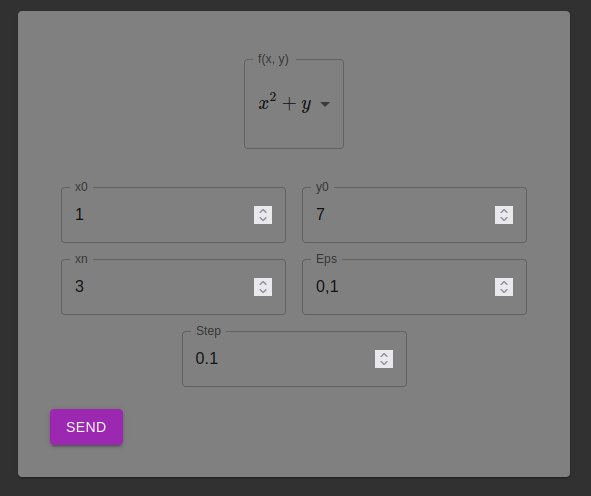
\includegraphics[width=.9\textwidth]{inp.jpg}\\
    \textbf{Рисунок 1: Ввод}
\end{center}

\begin{center}
    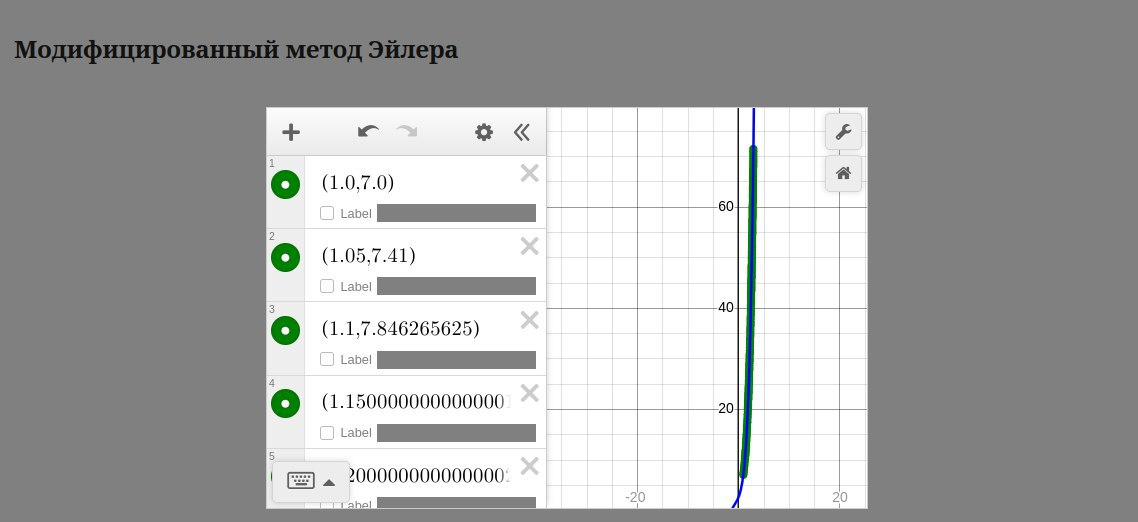
\includegraphics[width=.9\textwidth]{euler.jpg}\\
    \textbf{Рисунок 2: Модифицированный Эйлер}
\end{center}

\begin{center}
    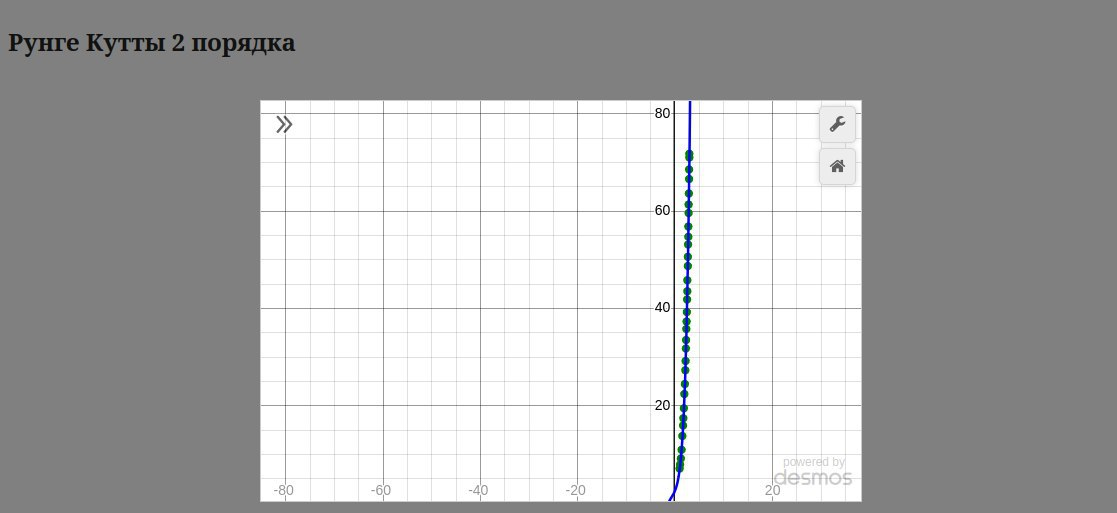
\includegraphics[width=.9\textwidth]{rung.jpg}\\
    \textbf{Рисунок 3: Рунге-Кутты 2}
\end{center}

\begin{center}
    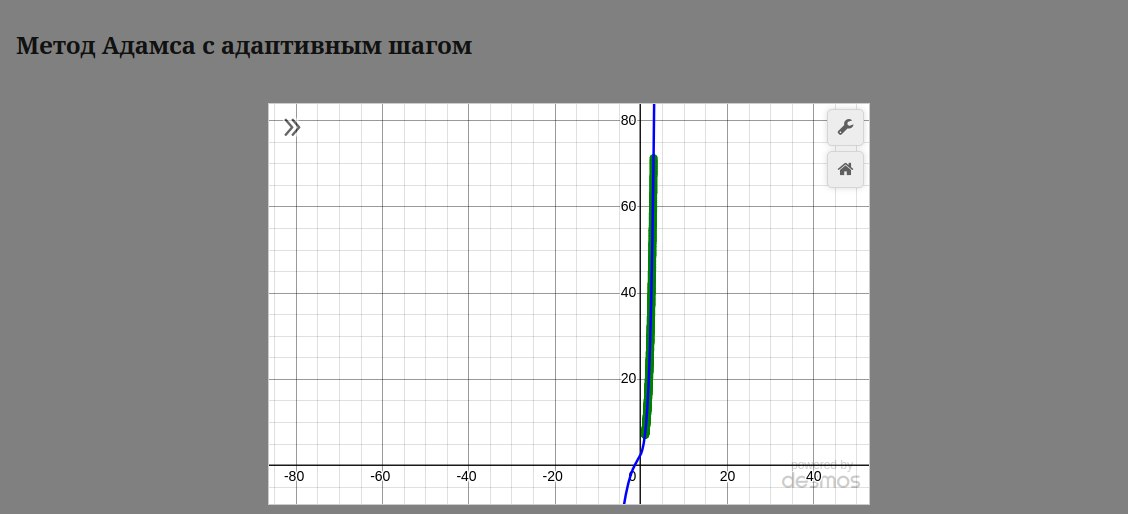
\includegraphics[width=.9\textwidth]{adams.jpg}\\
    \textbf{Рисунок 4: Адамс}
\end{center}

\section{Схемы}
\begin{center}
    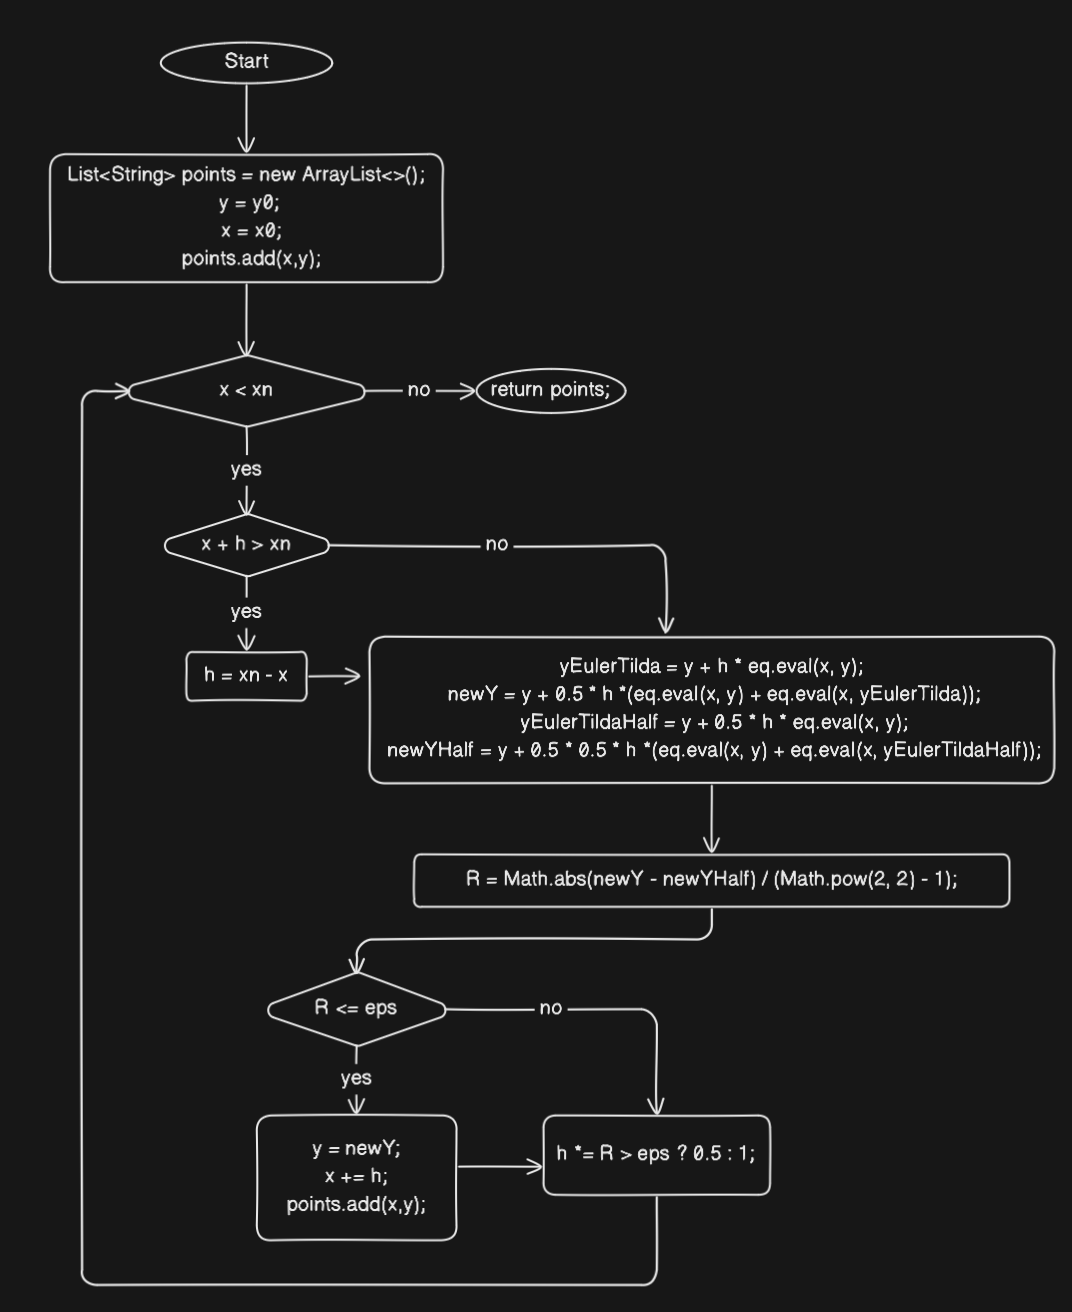
\includegraphics[width=.9\textwidth]{eulerS.png}\\
    \textbf{Схема 1: Модифицированный Эйлер}
\end{center}
\begin{center}
    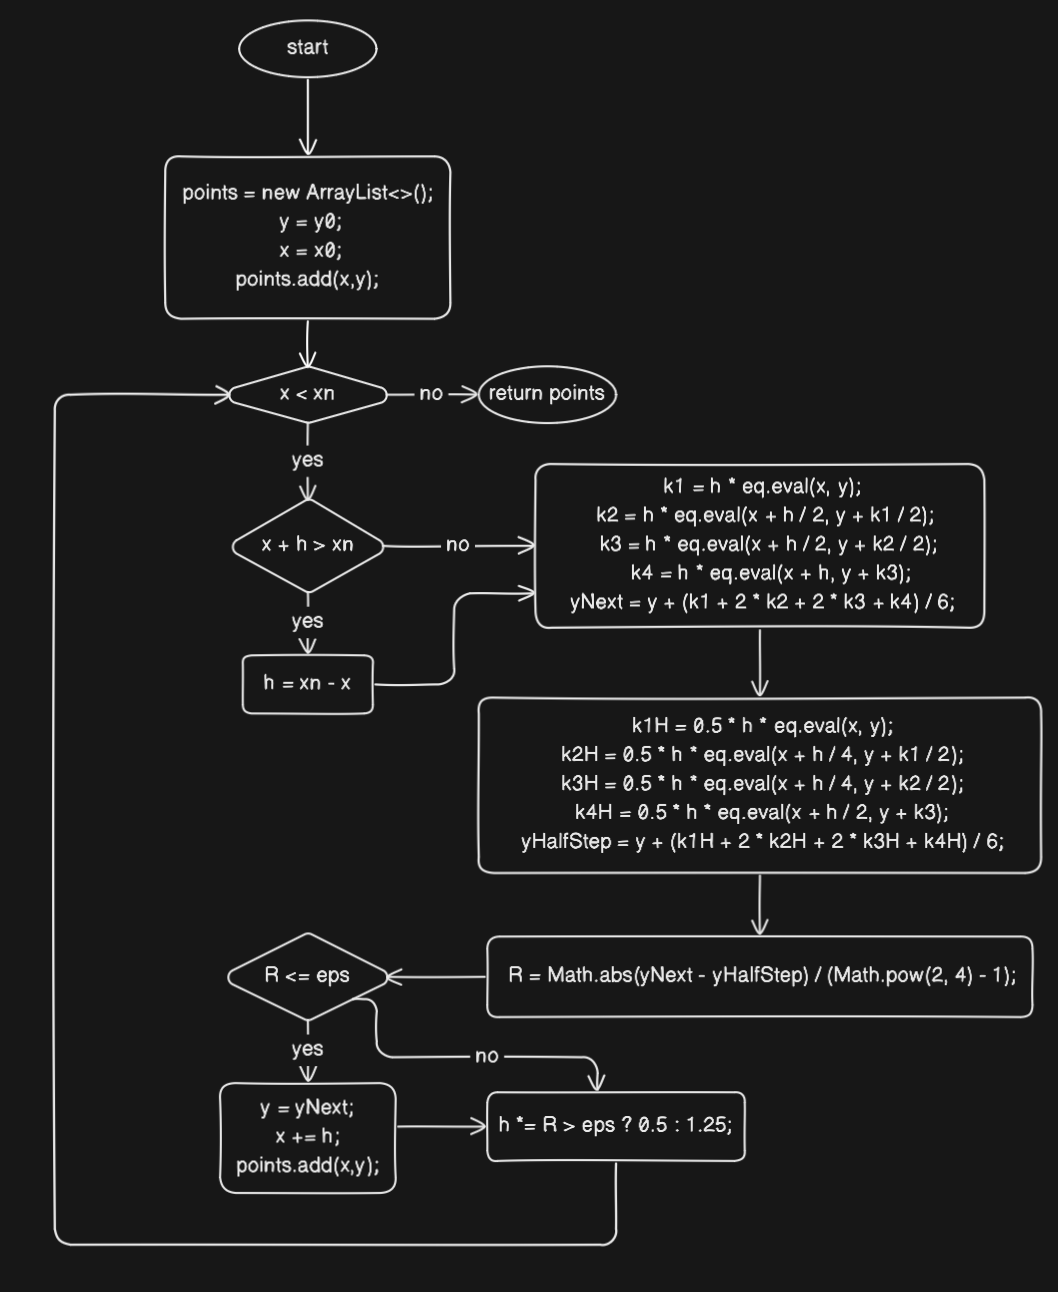
\includegraphics[width=.9\textwidth]{rungeS.png}\\
    \textbf{Схема 2: Рунге-Кутты 2}
\end{center}
\begin{center}
    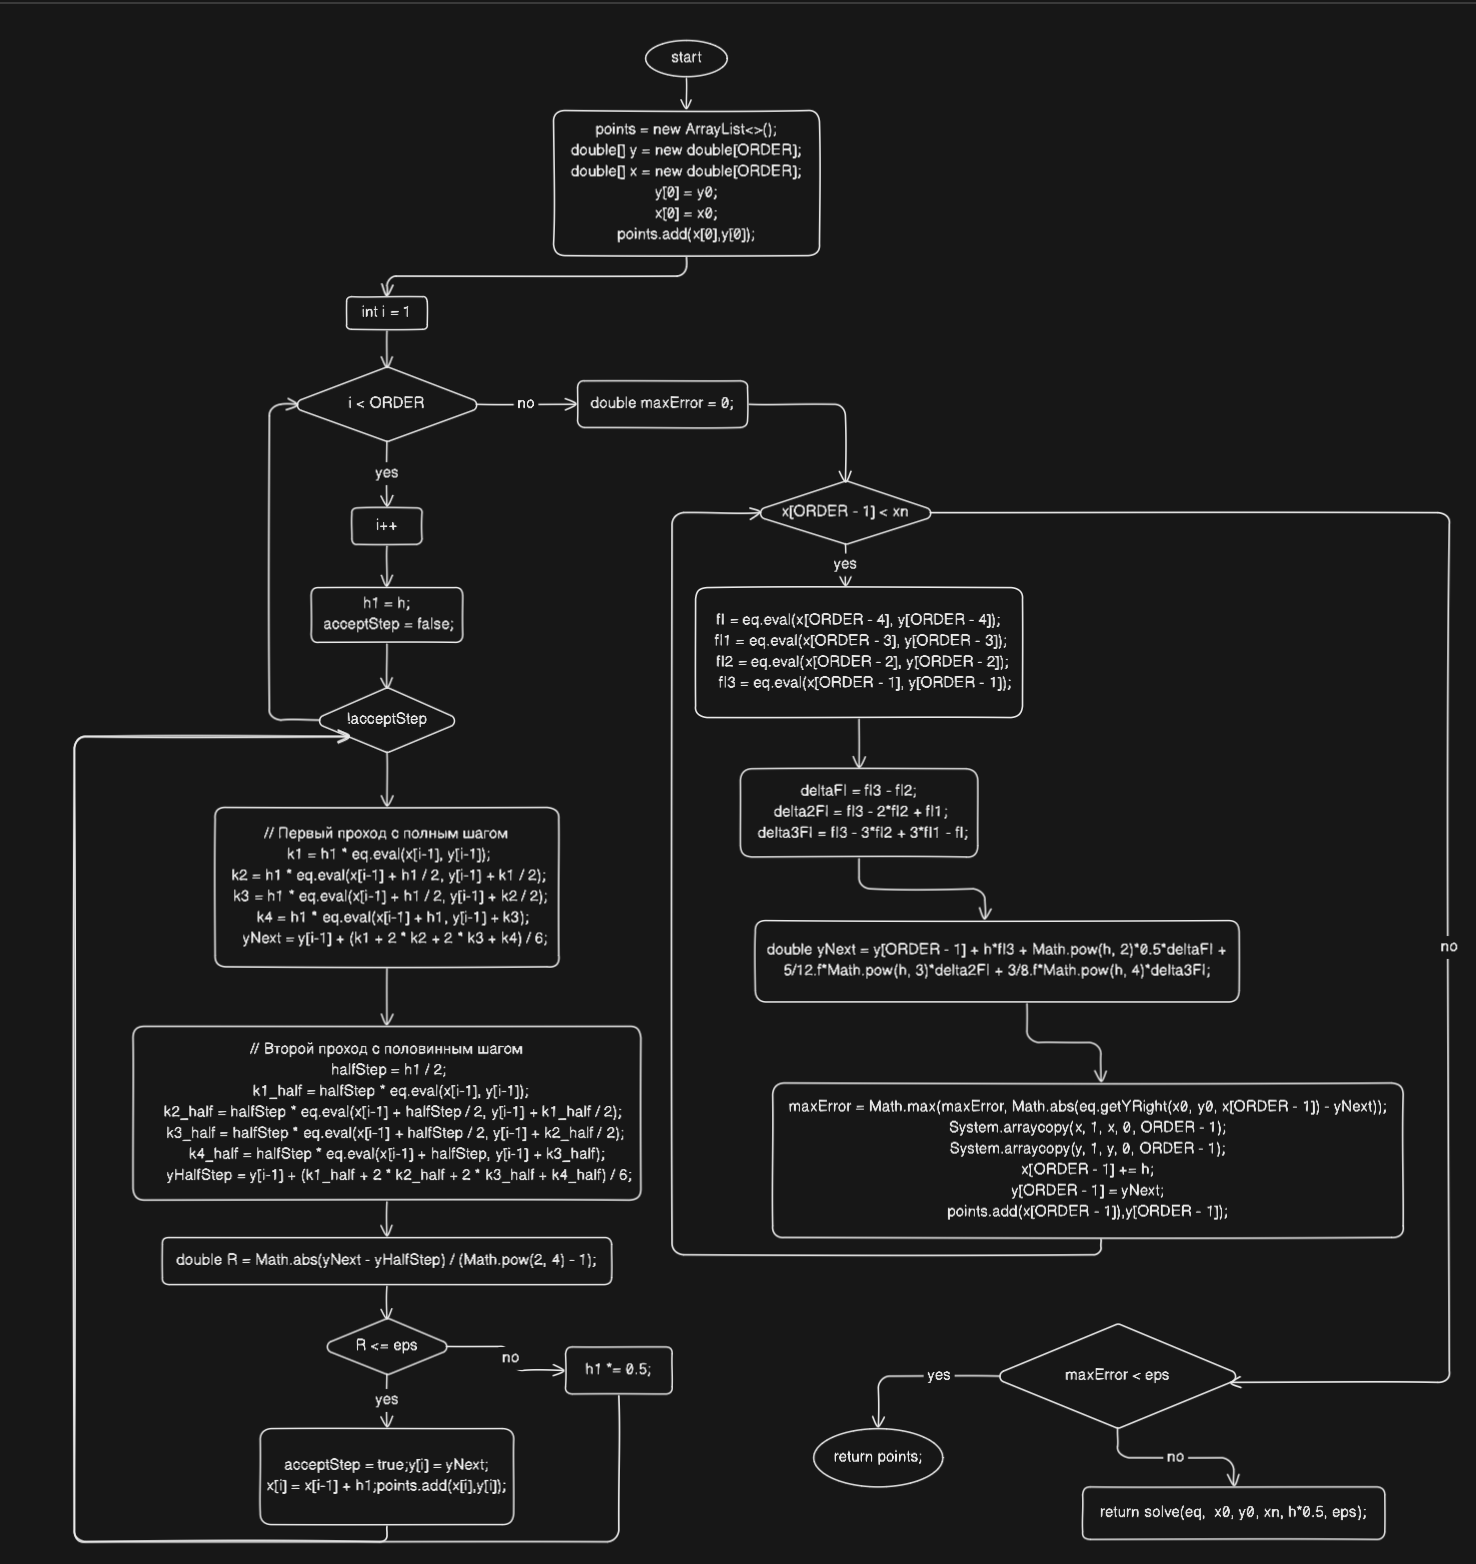
\includegraphics[width=.9\textwidth]{adams.png}\\
    \textbf{Схема 3: Адамс}
\end{center}

\section{GitHub}
Ссылка на мой репозиторий на GitHub: \url{https://github.com/Alex-de-bug/cm_math/tree/main/lab6}.

\section{Вывод}
В программе численные методы решения обыкновенных
дифференциальных уравнений (ОДУ) реализовали в
виде отдельного класса;
Для исследования использовали одношаговые методы и
многошаговые методы.
Для оценки точности одношаговых методов использовали правило
Рунге. Для оценки точности многошаговых методов использовали точное
решение задачи. Построить графики точного решения и полученного приближенного
решения.

\end{document}

\begin{center}
    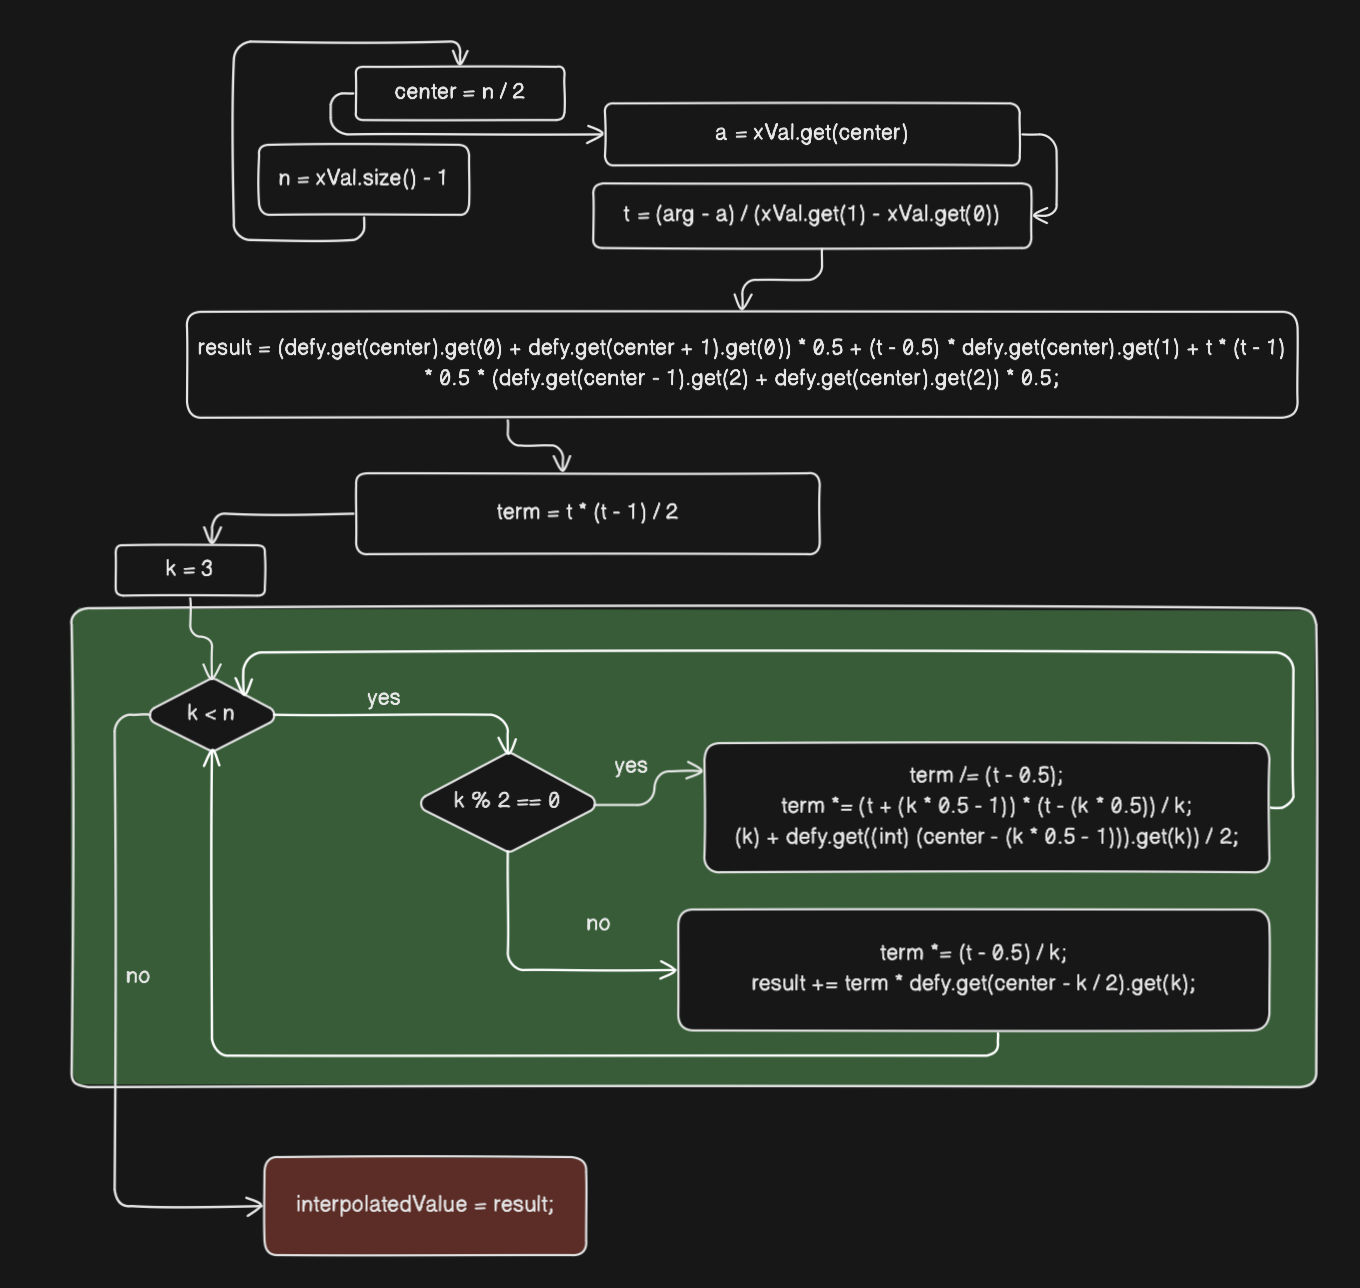
\includegraphics[width=.9\textwidth]{bessel.png}\\
    \textbf{Схема 5: Бессель}
\end{center}